\section{Question}

\begin{figure*}[!h]
    \center
    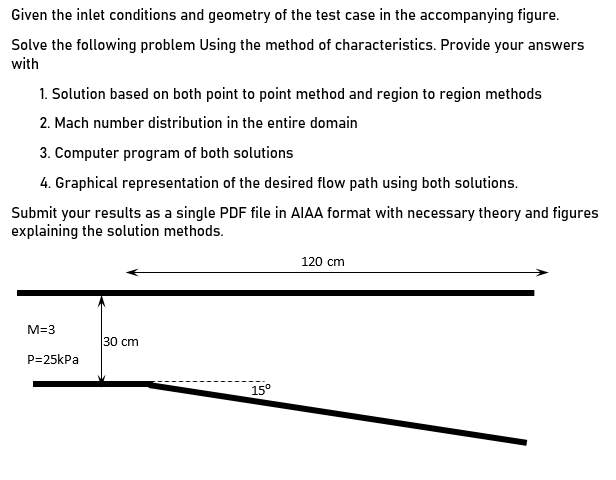
\includegraphics[scale=0.5]{results/question.png}
\end{figure*}

\textbf{SOLUTION:}\\

\par Given data
\begin{align*}
    M_1 &= 3.0 \\
    h &= 0.3 \ m \\
    L &= 1.2 \ m \\
    P_1 &= 25 \ kPa
\end{align*}

\par The solution algorithm followed for this problem is given below.\\

\par The number of characteristic nodes N, in the inlet plane is first chosen. The
value chosen for this problem is 100. An example layout of Characteristic lines
with N = 6, in the expansion flow domain of deflection angle $2^{\circ}$ is given in
\Cref{domain_layout}.But, the actual problem with $15^{\circ}$ deflection angle
requies N = 100 in order to accurately capture the expansion flow field. \\

\begin{figure}
   \center
    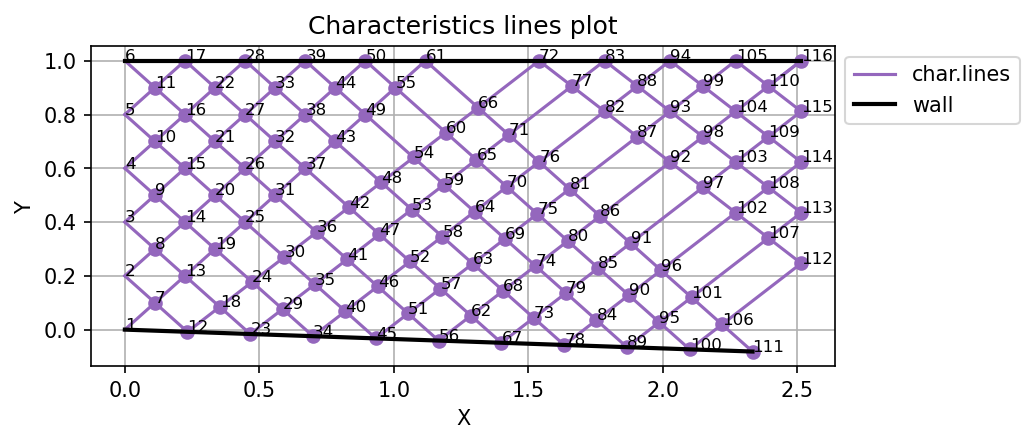
\includegraphics[scale=0.9]{results/expansion_corner_trial/char_map.png}
    \caption{Coarse characteristic points layout on the $2^{\circ}$ expansion corner}
    \label{domain_layout}
\end{figure}

\par Then the total number of characteristic nodes that will appear after all
interactions is computed using the equation below. Here, $n_{wall}$ is the number
of wall bounces requried as it is the one that controls the length of the
computation domain in this case. \\
\begin{align*}
    N_{total} = n_{wall} (2 N - 1) + N
\end{align*}

\par After this, a list of numbers indicating the characteristic points were
generated linearly similar to the one shown in \Cref{domain_layout} and the
points on both top and bottom wall is identified using the below equations
and were grouped for ease of computation.
\begin{align*}
    bottom\ wall: n_b = n_{b,prev} + (2N -1) \\
    top\ wall: n_b = n_{b,prev} + (N -1) \\
\end{align*}

\par Then a table, with the list of dependence upstream characteristic points,
to each internal and boundary char.point is made, which will be used during
computations. The inlet condition is defined such that, the expansion function
values $\nu(M)$ at all inlet char.points is computed for the following specified
condition. And the values of $K_1$ and $K_2$ were computed using the relations
given.
\begin{align*}
    M_{inlet} &= 3.0  \\
    \theta_{inlet} &= 0.0 \\
    K_1 &= \nu + \theta \\
    K_2 &= \nu - \theta
\end{align*}

\par Then the computation is begun for internal points, where the values of
$\nu$ and $\theta$ were computed by taking the intersected $K_1$ and $K_2$
upstream values as shown below.
\begin{align*}
    \nu &= \frac{K_1 + K_2}{2} \\
    \theta &= \frac{K_1 - K_2}{2}
\end{align*}

\par At the wall points, only one upstream characteristics meet, but the
wall angle $\theta_{wall}$ is known, hence using the upstream characteristic
and wall angle values, the expansion function is computed as shown in the
example below.
\begin{align*}
    bottom\ wall: \nu &= K_1 - \theta \\
    top\ wall: \nu &= K_2 + \theta
\end{align*}

\par Then, the Mach numbers at each characteristic point were computed using
Prandtl-Meyer expansion function relation given below.
\begin{align*}
    \nu(M) = \sqrt{\frac{\gamma+1}{\gamma-1}}tan^{-1}\sqrt{\frac{\gamma-1}{\gamma+1}\left(M^2-1\right)} - tan^{-1}\sqrt{M^2-1}
\end{align*}

\par For computing the location of downstream char.point, the following equations
that determine the slope of line (with the assumption that the char. curves are
straight lines in short length) and the location of the point as shown in the
\Cref{slope_image}.
\begin{figure}
    \center
    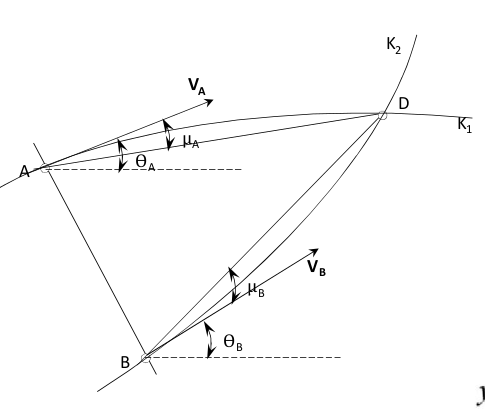
\includegraphics[scale=0.5]{results/slopeImage.png}
    \caption{reference image for the char. point position calculations}
    \label{slope_image}
\end{figure}


\begin{align*}
    \left(\frac{dy}{dx}\right)_A &= tan(\theta-\mu)_A \\
    \left(\frac{dy}{dx}\right)_B &= tan(\theta+\mu)_B \\
    S_1 &= \frac{tan(\theta-\mu)_A + tan(\theta-\mu)_B}{2} \\
    S_2 &= \frac{tan(\theta+\mu)_A + tan(\theta+\mu)_B}{2} \\
    y_D &=y_A + (x_D - x_A) S_1 \\
    y_D &=y_B + (x_D - x_B) S_2 \\
    x_D &= \frac{(S_2 x_B - S_1 x_A) + (y_A - y_B)}{S_2-S_1}
\end{align*}

\pagebreak
\textbf{Results:}

The Python code was developed for this computation and given in \Cref{appendixA}.
The contour of Mach number distribution and the characteristic points
obtained for this problem is given in \Cref{Mach_contour,char_output}, respectively. \\
\begin{figure}
    \center
    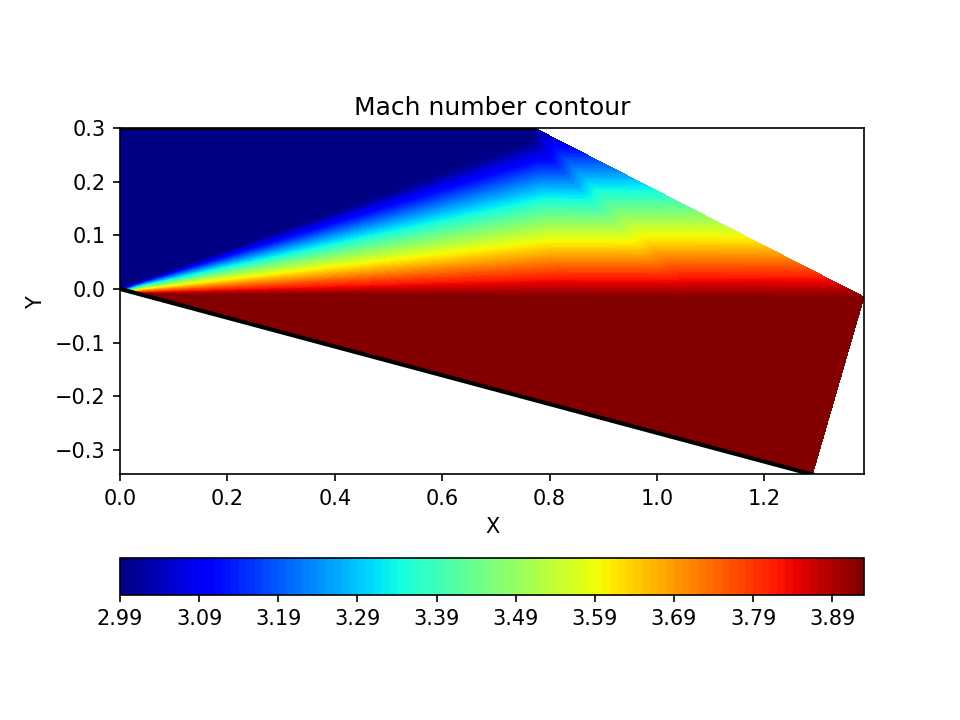
\includegraphics[scale=0.9]{results/expansion_corner/M_contour.png}
    \caption{Mach number contour output from computation}
    \label{Mach_contour}
\end{figure}

\begin{figure}
    \center
    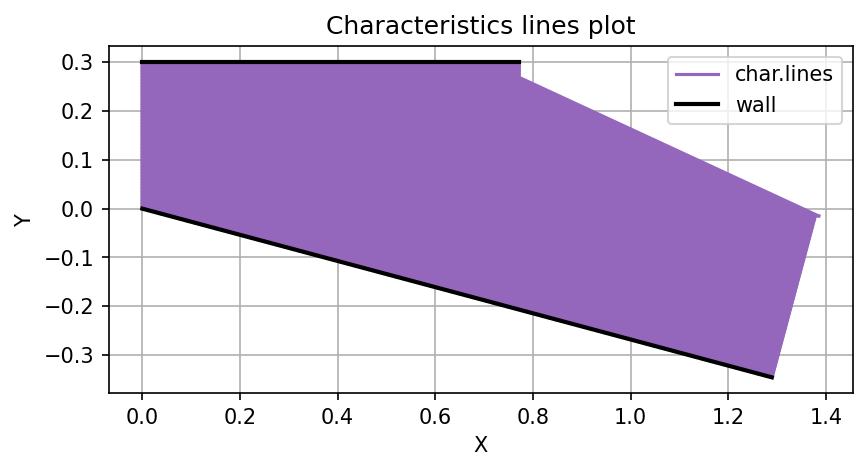
\includegraphics[scale=0.9]{results/expansion_corner/char_map.png}
    \caption{characteristic points distribution (conjested due to 18k points for N = 100)}
    \label{char_output}
\end{figure}

\par Further, the Mach number of downstream section after expansion, obtained
from the computation is compared with the theoretical value obtained
from \cite{ref_1}. The following gives the values obtained and they found to
be in agreement with the theory.
\begin{align*}
    M_{2,computation} &= 3.92329 \\
    M_{2,theory} &= 3.923
\end{align*}

\pagebreak
